\documentclass[11pt, a4paper]{article}
\usepackage{fullpage}
\usepackage[utf8]{inputenc}
\usepackage[T1]{fontenc}
\usepackage{graphicx}
\usepackage{float}
\usepackage{../tikz-uml}
\usepackage{amsmath}
\usepackage{amssymb}
\usepackage{listings}
\usepackage{hyperref}

\hypersetup{
    colorlinks=true,
    linkcolor=blue,
    filecolor=magenta,      
    urlcolor=cyan,
    pdftitle={Sharelatex Example},
    bookmarks=true,
    pdfpagemode=FullScreen,
}

\title{Apprentissage par renforcement multi-agents, De SlimeVolley à la RoboCup : Représentation d'un environnement avec Gym}
\author{Pélagie Alves\and Elias Debeyssac\and Alexis Hoffmann\and
Alexis Lhéritier\and Nicolas Majorel\and Sébastian Pagès}
\date{Février 2021}

\begin{document}

\maketitle

\newpage

\tableofcontents

\newpage


\section{Représentation d'un environnement avec Gym}


Il y a deux concepts clés dans l'apprentissage par renforcement, l'environnement et l'agent. (voir Apprentissage par renforcement pour les définitions).
Gym fournit principalement une abstraction de la représentation d'un environnement \cite{1606.01540} avec l'interface Env, il faut donc implémenter cette interface pour pouvoir créer un 
environnement et interagir avec celui-ci , respecter les consignes de la documentation \cite{core.py} pour qu'il soit correctement interprétable par les
différents algorithmes disponibles dans la bibliothèque stable\_baselines.\\
En revanche, Gym laisse la liberté à l'utilisateur de représenter un agent de la manière dont il souhaite, il n'y a pas de restrictions. \\

\noindent Il faut définir plusieurs attributs de base qui sont réutilisés dans les algorithmes d'apprentissage par renforcement pour déterminer l'action la plus adéquate, par exemple
pour l'algorithme PPO qui cherche à optimiser la politique, une règle utilisée par un agent pour décider des actions à entreprendre.\\

\subsection{ \textbf{Attributs à définir}} 
\begin{itemize}
	\item L'\textbf{espace d'observations} (observation\_space). 
	\item L'\textbf{espace d'actions} (action\_space). 
\end{itemize}

\noindent Ces espaces sont representés par des classes concrètes \cite{observation-and-action-spaces} implémentant l'interface Space \cite{space.py} du module Gym.

\begin{figure}[H]
    \centering
    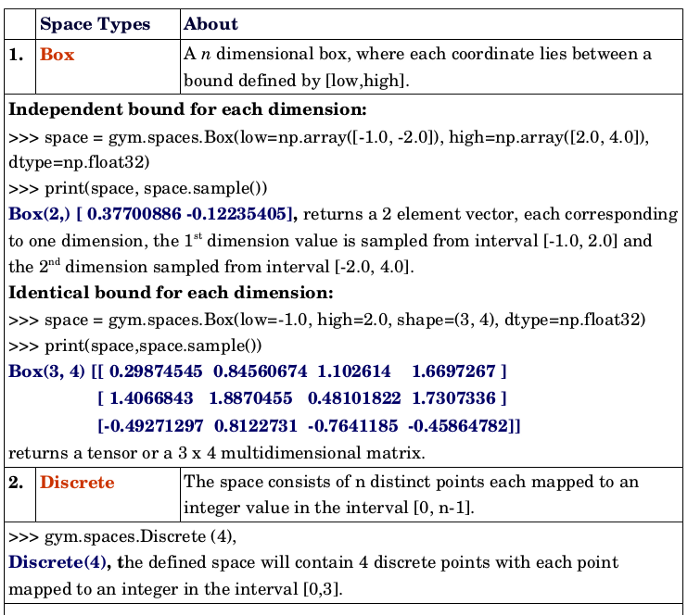
\includegraphics[scale=0.5]{../images/space1.png}
    \caption {description}
\end{figure}

\begin{figure}[H]
    \centering
    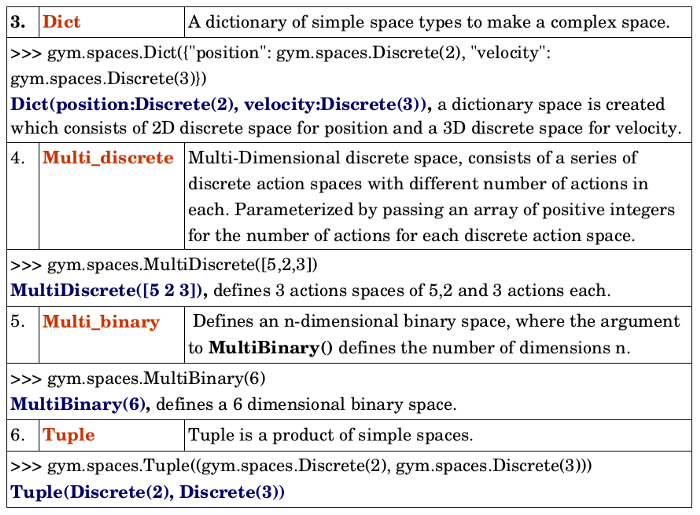
\includegraphics[scale=0.5]{../images/space2.png}
    \caption {description}
\end{figure}

\noindent Tel que précisé dans la documentation de gym , il est préférable d'éviter les versions différentes d'espaces et réutiliser les espaces existants spécifiés dans l'interface Space du module Gym pour permettre 
la comptabilité avec la plupart des modèles. \\

\subsection{ \textbf{Méthodes à implémenter\cite{openaigym}}} 

\begin{itemize}
  \item \textbf{step(self, action)}: 
  
  La fonction accepte une action fournie par l'agent et retourne un tuple \textit{(observation, reward, done, info)}. 

  Entrées :
  \begin{itemize}
	\item action : une action fournie par l'agent
  \end{itemize}	
  Sorties :
  \begin{itemize}
		\item observation(object): observation de l'agent dans l'environnement actuel.
		\item reward(float) : montant de la récompense retournée après l'action précédente.
		\item done(bool): si l'épisode est terminé, dans ce cas, plusieurs appels à la suite de cette fonction peuvent engendrer des comportements indéterminés.
		\item info(dict) : contient des informations auxiliaires.
  \end{itemize}	

	\item \textbf{reset(self)}: 
	
  	Réinitialise l'environnement à son état initial et renvoie une observation de cet état. \\
  	Cette fonction ne doit pas réinitialiser le générateur de nombres aléatoires de l'environment (graine, seed). \\
	Les variables aléatoires dans l'état de l'environnement doivent	être échantillonnées indépendamment entre plusieurs appels à `reset ()`. 
	En d'autres termes, chaque appel de `reset ()` devrait produire un environnement convenable pour
	un nouvel épisode, indépendant des épisodes précédents.

	Sorties :
	\begin{itemize}
		  \item observation(object): l'observation initiale.
	\end{itemize}	

	\item \textbf{close(self)}:
	Permet de détruire l'environnement. \\

	\item \textbf{seed(self, seed=None)}:
	
	Définit la graine pour le(s) générateur(s) de nombre aléatoires de cet environnement.

\end{itemize}

Ci-dessous, un exemple simple d'utilisation de l'environnement Gym: \\

\begin{figure}[H]
    \centering
    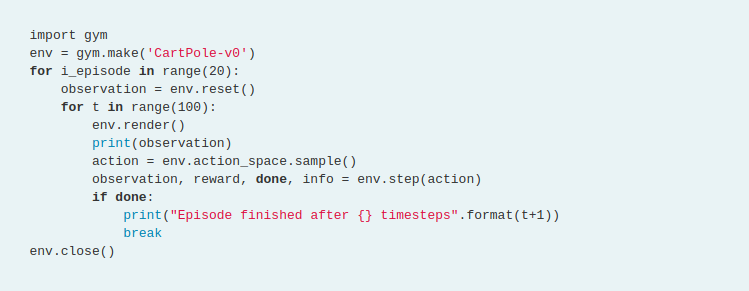
\includegraphics[scale=0.5]{../images/gym_example.png}
    \caption {description\cite{openaigymGit}}
\end{figure}



\section{Représentation de l'environnement SlimeVolleyBall} 



\subsection{\textbf{Éléments de l'environnement}}
\begin{itemize}
  \item Les éléments fixes : on distingue le filet, le sol et les bordures de la fenêtre, plus
  concrètement ces éléments définissent le perimètre de jeu des slimes et de la balle.\\
  Seulement le filet est un objet à part entière avec des coordonnées, une largeur et une hauteur. Le sol et les bordures de la fenêtre sont des 
  variables pour contrôler le périmètre de l'espace de jeu.
  
   \item Les éléments dynamiques : les slimes et la balle (coordonnées, dimensions, vitesse), parmi ces éléments seulement les slimes sont des agents, la balle ne décide pas de l'action
   à effectuer, elle n'interprète pas l'environnement pour modifier sa trajectoire, il n'y a pas non plus de notions de récompenses pour celle-ci, 
   elle suit seulement une trajectoire qui dépend de sa vitesse et des interactions avec l'environnement.\\
   Par défaut, l'agent que l'on entraîne est celui à droite, l'agent à gauche est contrôlé par un réseau de neurones \cite{ha2015slimevolley} (jeu JavaScript de 2015).

   \item Le générateur de nombres aléatoires : dans SlimeVolleyBall, à chaque nouvelle manche, la balle est propulsée depuis une position fixe du terrain à une certaine vitesse. Cette vitesse est déterminée
   par une séquence prédéfinie de paramètres dépendant de la graine (seed) utilisée. 
   L'idée d'utiliser une graine est de pouvoir répéter exactement le même environnement, mais avec des politiques d'actions différentes des agents pour comparer
   les résultats.
  
  \end{itemize}

  \begin{figure}[H]
    \centering
    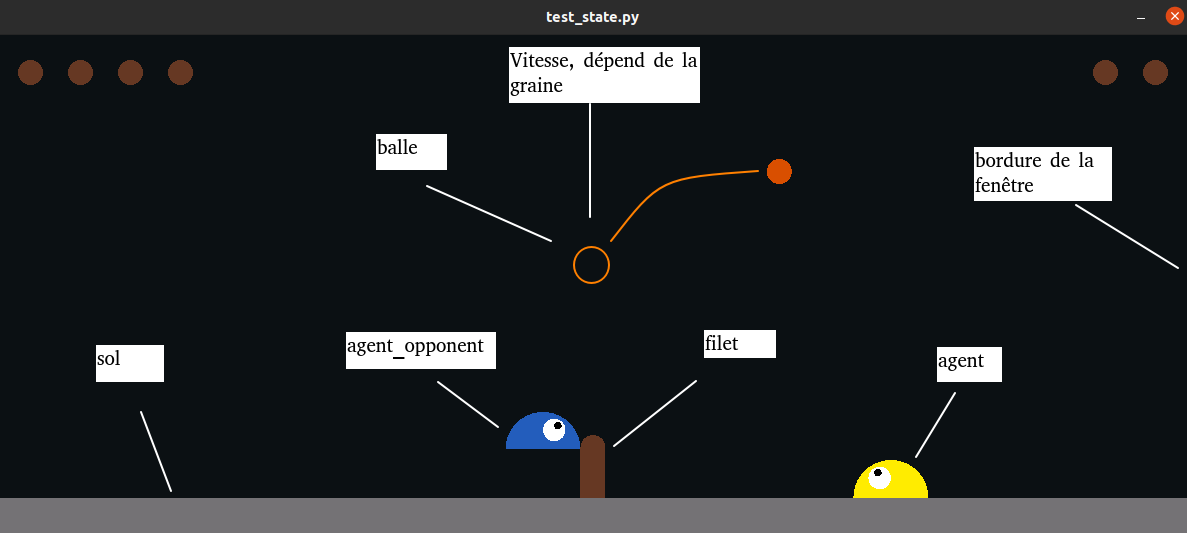
\includegraphics[scale=0.5]{../images/schema.png}
    \caption {description}
\end{figure}

\subsection{\textbf{Types d'environnement}} 

  \noindent On distingue trois types d'environnement dans le jeu SlimeVolleyBall.

	\begin{figure}[H]
		\centering
		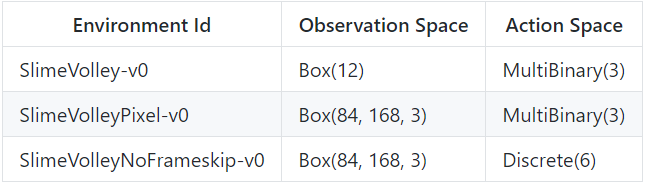
\includegraphics{../images/environnementsS.PNG}
		\caption {différents environnements de SlimeVolleyGym}
	\end{figure}

  \noindent L'environnement \textit{SlimeVolley-v0} correspond à un environnement avec un \textbf{mode d'observation par états}. \\
  L'environnement \textit{SlimeVolleyPixel-v0} correspond à un environnement avec un \textbf{mode d'observation par pixels}. \\
  L'environnement \textit{SlimeVolleyNoFrameskip-v0} correspond à un environnement avec un \textbf{mode d'observation par pixels (Atari)}. \\

  \noindent Le mode d'observation par pixels (Atari) encapsule en fait les comportements du mode d'observation par pixels. Les deux environnements travaillent
  sur les mêmes données d'observation. \\
  Cependant, les scripts pour entraîner le modèle dans le code base n'utilisent pas le mode d'observation par pixels mais plutôt le mode d'observation par pixels (Atari).

  \noindent On détaillera par la suite ces différentes espaces. \\

  \subsection{\textbf{Espaces d'observations}} 

  \begin{itemize}
 
  \item\textbf{Mode d'observation par états} :  Les deux agents et la balle sont representés par un vecteur à 12 dimensions : 
	
		$$
	\begin{bmatrix}
		x\_agent & y\_agent & \dot{x} \_agent & \dot{y}\_agent \\
		x\_ball & y\_ball & \dot{x}\_ball & \dot{y}\_ball \\
		x\_opponent & y\_opponent & \dot{x}\_opponent & \dot{y}\_opponent \\
	\end{bmatrix}
	\quad
	$$

	Ici, x représente la coordonnée abscisse, y la coordonnée ordonnée, $\dot{x}$ la vitesse en abscisse, $\dot{y}$ la vitesse en ordonnée.

	Cet espace est représenté par un objet de type \textit{Box} (implémentation de la classe Space du module gym), cet espace représente une "boîte" à n dimensions.
	Ici, chaque paramètre de la matrice à un intervalle de valeurs acceptées (valeurs basses et hautes).\\
	
	Ce mode d'observation est utilisé dans l'environnement SlimeVolley-v0.

	\begin{center}
	\begin{tabular}{ |c|c|c|c|c|c| }
	
	\hline
	observation    & $x\_agent$ & $y\_agent$ & $\dot{x} \_agent$ & $\dot{y} \_agent$ & ...\\ 
	min & -3.4028235e+38 & -3.4028235e+38 & -3.4028235e+38 & -3.4028235e+38 & ...\\  
	max & 3.4028235e+38 & 3.4028235e+38 & 3.4028235e+38 & 3.4028235e+38 & ...  \\
	\hline
	\end{tabular}
	\end{center}
	
	\begin{lstlisting}[language=python, frame=single, gobble=8, tabsize=4]	
		import numpy as np
		from gym import spaces

			high = np.array([np.finfo(np.float32).max] * 12)
			self.observation_space = spaces.Box(-high, high)
		
	\end{lstlisting}	

  \item\textbf{Mode d'observation par pixels (Atari) } 
  
  
  Entraîner un agent à jouer au Slime Volleyball uniquement à partir d'images pixelisées est plus difficile, car l'agent doit travailler avec un espace d'observations plus grand, 
  mais il doit surtout apprendre à déduire les informations importantes dans les images telles que les position des agents, de la balle, les vitesses qui ne sont pas explicitement fournies. Pour obtenir ces informations, on doit pré-traiter les images du mode d'observations par pixels. \\\\
  Le pré-traitement standard Atari \cite{TRAINING.md} pour les agents consiste d'abord à convertir chaque image RGB en échelle de gris (on passe de 3 valeurs R = 0-255, G = 0-255, B = 0-255 à une seule valeur de 0-255), à les redimensionner en 84x84 pixels (84x168 à la base), 
  ensuite, 4 images consécutives sont empilées en une seule observation afin que les informations temporelles locales puissent être déduites.\\

	
 \begin{figure}[H]
    \centering
    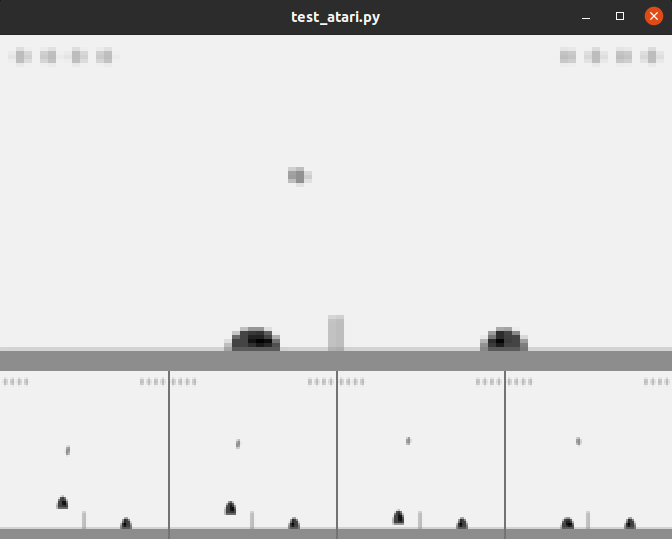
\includegraphics[scale=0.5]{../images/atari.png}
    \caption {Environnement SlimeVolleyNoFrameskip-v0}
\end{figure}
 
  Cet environnement est représenté par un objet de type \textit{space.Box}, une matrice de dimensions 84 pixels en hauteur, 168 en largeur en RGB. Il a la particularité de montrer le fonctionnement du pré-traitement des images décrit.\\

Ce mode est utilisé dans l'environnement SlimeVolleyPixel-v0 et SlimeVolleyNoFrameskip-v0.

\noindent Pour de plus amples informations, il faut se diriger vers le script \textbf{test\_atari} \cite{test-atari.py} qui crée un environnement SlimeVolleyBall Atari
	compatible. \\



	\begin{lstlisting}[language=python, frame=single, gobble=8, tabsize=4]	
		from gym import spaces

			self.observation_space = spaces.Box(low=0, high=255,
	  		shape=(PIXEL_HEIGHT, PIXEL_WIDTH, 3), dtype=np.uint8)
	\end{lstlisting}

\end{itemize}

\subsection{\textbf{Espaces d'actions}}

\noindent L'espace d'action est soit de type Multibinary soit de type Discrete.\\\\
Dans le mode MultiBinary on a un espace d'action représenté par un vecteur de booléens à 3 dimensions avec les champ avancer, reculer, sauter (droite, gauche, haut). La valeur est à 1 si l'action est demandée, 0 dans le cas contraire.

  \begin{lstlisting}[language=python, frame=single, gobble=4, tabsize=4]	
	from gym import spaces
	self.action_space = spaces.MultiBinary(3)
\end{lstlisting}


  $$
  \begin{bmatrix}
      $avancer = 1$ & $reculer = 0$ & $sauter = 1$  \\
  \end{bmatrix}
  \quad
  $$

  \noindent Dans l'exemple ci dessus, le slime fait un saut en avant.\\


\noindent Dans le mode Discrete on a un espace d'action représenté par un vecteur d'entier de 0 à 5, chaque action correspond à un chiffre (0=immobile, 1=avancer, 2=saut avant, 3=saut, 4=saut arrière, 5=reculer).


\noindent Le mode MultiBinary est utilisé dans SlimeVolley-v0 et SlimeVolleyPixel-v0.\\
Le mode Discrete est utilisé dans SlimeVolleyNoFrameskip-v0.


\subsection{\textbf{Affichage}} 

\noindent On illustre ici, un exemple d'implémentation de la méthode \textbf{render(self, mode='human')} de l'interface Env.\\\\ Pour stocker les éléments visuels d’une forme géométrique, 
l'implémentation choisie par le créateur de SlimeVolleyGym est de créer une variable canvas qui va permettre de représenter diverses
formes géométriques (rectangle, cercle, demi-cercle).\\
En fonction du mode d'observations (états, pixels), le type du canvas est différent. \\
Ci-dessous les fonctions à appeler pour créer et modifier un canvas dans le programme :\\
		
\begin{lstlisting}[language=python, frame=single, gobble=8, tabsize=4]	
	def create_canvas(canvas, c):
	def rect(canvas, x, y, width, height, color):
	def half_circle(canvas, x, y, r, color):
	def circle(canvas, x, y, r, color):
\end{lstlisting}

\begin{itemize}

	\item \textbf{Affichage : observations par états} : \\
	
	\noindent Dans le cadre de l'\textbf{observations par états}, le canvas est créé en tant que \textbf{Viewer} object \cite{rendering.py} (Objet natif de gym). 
	Un Viewer object permet par exemple de créer un rectangle à partir de sa largeur et de sa hauteur. Le rectangle est tracé 
	depuis le point en haut à gauche de celui-ci.\\
	Un exemple d'utilisation pour créer un rectangle et l'afficher :\\
	
	\begin{lstlisting}[language=python, frame=single, gobble=4, tabsize=4]
		
	from gym.envs.classic_control import rendering as rendering

		canvas = rendering.Viewer(WINDOW_WIDTH, WINDOW_HEIGHT)
		box = rendering.make_polygon([(0,0), (0,-height), 
		(width, -height), (width,0)])
		# ...
		canvas.add_onetime(box)
		canvas.render(return_rgb_array = mode=='rgb_array')
	\end{lstlisting}



	\item \textbf{Affichage : observations par pixels} : \\
	
	\noindent Pour le mode d'\textbf{observations par pixels}, le canvas contient une matrice de dimensions [3 n] avec n le nombre de pixels de l’objet et 3 pour chaque valeur RGB de l’image. \\ Exemple : \\

	$$
	\begin{bmatrix}
	0|12|5 & 145|44|88 & 168|11|3 & 27|255|0 & 42|99|4 \\ 
	102|88|11 & 0|14|24 & 127|122|211 & 35|44|77 & 2|43|44 \\ 
	64|64|64 & 42|1|2 & 24|4|9 & 18|255|254 & 0|1|255 \\ 
	\end{bmatrix}
	\quad
	$$ \\
	Les données affichées sont en fait similaires aux données utilisées pour l'observation. \\\\
	Le programme utilise le module \textbf{OpenCV} \cite{OpenCV}, celui-ci permet de représenter des formes géométriques sous forme de matrices, mais également réaliser des opérations mathématiques sur des images 
	(retourner, réduire l'image), toutes les structures de tableaux OpenCV sont converties vers et à partir de tableaux Numpy. \\ \\
	Initialisation du canvas dans le programme : \\
	\begin{lstlisting}[language=python, frame=single, gobble=4, tabsize=4]
	import numpy as np	
		background_color = (11, 16, 19)
		canvas = np.ones((WINDOW_HEIGHT, WINDOW_WIDTH, 3), 
		dtype=np.uint8)
    	for background_color in range(3):
      		canvas[:, :, background_color] *= c[background_color]
	\end{lstlisting}

	\noindent Un exemple pour dessiner un rectangle sur le canvas : \\

	\begin{lstlisting}[language=python, frame=single, gobble=4, tabsize=4]	
	import cv2
		canvas = cv2.rectangle(canvas, (round(x), 
		round(WINDOW_HEIGHT-y)), (round(x+width),
		 round(WINDOW_HEIGHT-y+height)),
		color, thickness=-1, lineType=cv2.LINE_AA)
	\end{lstlisting}
	
	Le résulat est interprété avec l'objet \textbf{SimpleImageViewer} \cite{rendering.py} (Objet natif de gym) à partir de la matrice, on peut l'afficher ensuite : \\

	\begin{lstlisting}[language=python, frame=single, gobble=4, tabsize=4]	
	from gym.envs.classic_control import rendering as rendering
		self.viewer = rendering.SimpleImageViewer(maxwidth=2160)
		self.viewer.imshow(canvas)
	\end{lstlisting}

\end{itemize}

\subsection{\textbf{Exécuter une action dans l'environnement} }

\noindent Voici un exemple d'implémentation de la méthode \textbf{step(self, action)} de l'interface Env. \\ La méthode se contente principalement d'exécuter les actions des agents,
le paramètre \textit{action} contient l'action de l'agent de droite, comme spécifier plus haut de base l'agent de gauche est contrôlé par la politique de base du réseau de neurones (objet \textbf{BaselinePolicy} \cite{slimevolley.py}), 
cependant, on a également un hyperparamètre \textit{otherAction} qui permet de modifier le comportement de base de celui-ci et donc de changer l'action prédite en utilisant un autre algorithme.\\
Les actions sont donc envoyées au moteur interne du jeu (objet \textbf{Game} \cite{slimevolley.py}) qui va contrôler celles-ci (déplacement, gestion des collisions, marquage de points), la fonction qui contrôle
tout ce mécanisme renvoie le résultat \underline{selon la perspective de l'agent de droite} (donc 1 si celui-ci marque un point, -1 s'il perd un point, 0 s'il ne passe rien).\\
La méthode vérifie ensuite si un des deux agents n'a plus de vies ou si le temps maximum sans marquer de points est dépassé, dans ce cas, le jeu est terminé.\\
Finalement, la méthode retourne plusieurs informations, comme spécifier plus haut dans la partie "Représentation d'un environnement avec Gym".\\ \\
Plus précisément, un tuple avec les informations suivantes :
\begin{itemize}
	\item Un booléen pour indiquer si le jeu est terminé
	\item Les observations selon la perspective de l'agent de droite : 
		\begin{itemize}
			\item observation par états : même type de données renvoyées (voir "Mode d'observation par états"), cependant les informations renvoyées sont relatives par rapport à l'agent (voir objet 
			\textbf{RelativeState} \cite{slimevolley.py}), 
			"un agent jouant d'un côté ou de l'autre du terrain doit voir les observations de la même manière".
			\item obervations par pixels : renvoie la matrice qui est spécifiée dans la partie au dessus pour l'affichage.
		\end{itemize}
	\item La récompense selon la perspective de l'agent de droite
	\item Un tuple auxiliaire contenant :
		\begin{itemize}
		\item Nombres de vies restantes pour l'agent de droite
		\item Nombres de vies restantes pour l'agent de gauche
		\item Les observations selon la perspective de l'agent de gauche :
		 \begin{itemize}
			\item observation par états : relatives par rapport à l'agent de gauche.
			\item obervations par pixels : la matrice utilisée pour l'affichage est retournée avec la fonction flip du module \textbf{OpenCV}.
		 \end{itemize}
		\end{itemize}
	
	
\end{itemize}

\subsection{\textbf{Création et utilisation de la graine}} 

\noindent Pour créer un générateur de nombres aléatoires, l'implémentation de la méthode \textbf{seed(self, seed=None)} utilise le module \textbf{utils} de \textbf{Gym} pour créer une seed. \\

\begin{lstlisting}[language=python, frame=single, gobble=4, tabsize=4]	
	from gym.utils import seeding
		self.np_random, seed = seeding.np_random(seed)
		self.game = Game(np_random=self.np_random)
\end{lstlisting}


\noindent Ensuite, à partir de cette seed, on peut générer une séquence prédéfinie de vitesses pour la balle.

\begin{lstlisting}[language=python, frame=single, gobble=4, tabsize=4]	
	ball_vx = self.np_random.uniform(low=-20, high=20)
    ball_vy = self.np_random.uniform(low=10, high=25)
\end{lstlisting}




\section{Bibliographie}

\bibliographystyle{../elsarticle-num}
\bibliography{../Sources}


\end{document}
